\documentclass{article}

% content/resources/templates/preamble.tex
\usepackage[margin=0.6in]{geometry}
\author{Milav Dabgar}
\usepackage{amsmath,amssymb,amsthm}
\usepackage{booktabs}
\usepackage{multirow}
\usepackage{xcolor}
\usepackage{tcolorbox}
\tcbuselibrary{breakable,skins}
\usepackage[colorlinks=true,linkcolor=blue]{hyperref}
\usepackage{titlesec}
\usepackage{enumitem}
\usepackage{tikz}
\usepackage{pgfplots}
\usepackage{circuitikz}
\usepackage[version=4]{mhchem}
\usepackage{longtable}
\usepackage{array}
\usepackage{float}
\usepackage{caption}
\usepackage{listings}

\lstset{
  basicstyle=\small\ttfamily,
  breaklines=true,
  breakatwhitespace=false,
  postbreak=\mbox{\textcolor{red}{$\hookrightarrow$}\space},
  float=false,
  numbers=left,
  numberstyle=\tiny\color{gray},
  numbersep=10pt,
  xleftmargin=2em,
  keywordstyle=\color{blue},
  commentstyle=\color{green!60!black},
  stringstyle=\color{purple},
  backgroundcolor=\color{gray!5},
  showstringspaces=false,
  tabsize=2,
  captionpos=b,
  keepspaces=true,
  columns=flexible
}

\pgfplotsset{compat=1.18}
\usetikzlibrary{shapes,arrows,positioning,calc,patterns,decorations.pathmorphing,decorations.markings,arrows.meta}

% Color scheme
\definecolor{headcolor}{RGB}{0,102,204}
\definecolor{keycolor}{RGB}{220,20,60}
\definecolor{solutioncolor}{RGB}{34,139,34}
\definecolor{mnemoniccolor}{RGB}{148,0,211}
\definecolor{codecolor}{RGB}{0,0,100}

% Spacing
\setlength{\parskip}{3pt}
\setlist[itemize]{nosep}
\setlist[enumerate]{nosep}

% Title formatting
\titleformat{\section}{\Large\bfseries\color{headcolor}}{\thesection}{1em}{}
\titleformat{\subsection}{\large\bfseries\color{headcolor}}{\thesubsection}{1em}{}

% Pandoc tightlist compatibility
\providecommand{\tightlist}{%
  \setlength{\itemsep}{0pt}\setlength{\parskip}{0pt}}

% Pandoc longtable compatibility
\newcounter{none}
\def\thenone{}


% content/resources/templates/english-boxes.tex

% Custom environments
\newtcolorbox{solutionbox}{
 breakable,
 enhanced,
 colback=solutioncolor!5!white,
 colframe=solutioncolor!75!black,
 fonttitle=\bfseries,
 title=Solution
}

\newtcolorbox{solutionboxnobreak}{
 colback=solutioncolor!5!white,
 colframe=solutioncolor!75!black,
 fonttitle=\bfseries,
 title=Solution
}

\newtcolorbox{keyformula}{
 breakable,
 enhanced,
 colback=keycolor!5!white,
 colframe=keycolor!75!black,
 fonttitle=\bfseries,
 title=Key Formula
}

\newtcolorbox{mnemonicboxenv}{
 breakable,
 enhanced,
 colback=mnemoniccolor!5!white,
 colframe=mnemoniccolor!75!black,
 fonttitle=\bfseries,
 title=Mnemonic
}

\newcommand{\mnemonicbox}[1]{%
  \begin{mnemonicboxenv}
    #1
  \end{mnemonicboxenv}
}


% Custom commands for GTU solutions
% This file defines semantic commands for consistent formatting

% Question command with automatic formatting
\newcommand{\question}[2]{%
  \section*{Question #1}%
  \textbf{#2}%
}

% OR question variant
\newcommand{\questionor}[2]{%
  \section*{Question #1 OR}%
  \textbf{#2}%
}

% Proper table environment with caption
\newenvironment{answertable}[1]{%
  \begin{table}[htbp]
  \centering
  \caption{#1}
}{%
  \end{table}
}

% Proper figure environment for diagrams
\newenvironment{answerdiagram}[1]{%
  \begin{figure}[htbp]
  \centering
  \caption{#1}
}{%
  \end{figure}
}

% Semantic markup for key terms
\newcommand{\keyword}[1]{\textbf{#1}}
\newcommand{\code}[1]{\texttt{#1}}
\newcommand{\classname}[1]{\texttt{#1}}
\newcommand{\methodname}[1]{\texttt{#1}}

% Proper quotation marks
\newcommand{\mnemonic}[1]{``#1''}

\usetikzlibrary{mindmap,trees,shadows,backgrounds}

\title{Entrepreneurship and Start-ups (4300021) - Winter 2024 Solution}
\date{November 19, 2024}

\begin{document}
\maketitle

\questionmarks{1(a)}{3}{Distinguish between Entrepreneur and Manager.}

\begin{solutionbox}
\textbf{Answer}:

\begin{center}
\captionof{table}{Entrepreneur vs Manager}
\begin{tabulary}{\linewidth}{L L L}
    \toprule
    \textbf{Aspect} & \textbf{Entrepreneur} & \textbf{Manager} \\
    \midrule
    \textbf{Primary Role} & Creates new ventures and opportunities & Administers existing operations \\
    \textbf{Risk Taking} & High risk-taker, bears uncertainty & Low to moderate risk, follows guidelines \\
    \textbf{Decision Making} & Quick, intuitive decisions & Systematic, policy-based decisions \\
    \textbf{Focus} & Innovation and growth & Efficiency and control \\
    \textbf{Rewards} & Profit and ownership & Salary and benefits \\
    \bottomrule
\end{tabulary}
\end{center}
\end{solutionbox}

\begin{mnemonicbox}
\mnemonic{"CRIFO" - Creates Risk Innovation Focus Ownership}
\end{mnemonicbox}

\questionmarks{1(b)}{4}{Explain any four functions of Entrepreneurship.}

\begin{solutionbox}
\textbf{Answer}:

\begin{itemize}
    \item \keyword{Job Creation}: Entrepreneurs establish new businesses, creating employment opportunities for others
    \item \keyword{Innovation}: They introduce new products, services, or processes to meet market needs
    \item \keyword{Economic Development}: Generate wealth, contribute to GDP, and stimulate economic growth
    \item \keyword{Risk Taking}: Accept business uncertainties and financial risks for potential profits
\end{itemize}

\begin{center}
    \begin{tikzpicture}[node distance=1.5cm, auto]
        \node [gtu block] (Main) {Entrepreneurship Functions};
        \node [gtu block, below left=1.5cm and 0.5cm of Main] (Job) {Job Creation};
        \node [gtu block, below right=1.5cm and 0.5cm of Main] (Inn) {Innovation};
        \node [gtu block, left=of Job] (Eco) {Economic Development};
        \node [gtu block, right=of Inn] (Risk) {Risk Taking};

        \node [gtu state, below=0.5cm of Job] (JobDetail) {Employment Generation};
        \node [gtu state, below=0.5cm of Inn] (InnDetail) {New Products/Services};
        \node [gtu state, below=0.5cm of Eco] (EcoDetail) {GDP Growth};
        \node [gtu state, below=0.5cm of Risk] (RiskDetail) {Business Uncertainty};

        \draw [gtu arrow] (Main) -- (Job);
        \draw [gtu arrow] (Main) -- (Inn);
        \draw [gtu arrow] (Main) -- (Eco);
        \draw [gtu arrow] (Main) -- (Risk);
        \draw [gtu arrow] (Job) -- (JobDetail);
        \draw [gtu arrow] (Inn) -- (InnDetail);
        \draw [gtu arrow] (Eco) -- (EcoDetail);
        \draw [gtu arrow] (Risk) -- (RiskDetail);
    \end{tikzpicture}
    \captionof{figure}{Functions of Entrepreneurship}
\end{center}
\end{solutionbox}

\begin{mnemonicbox}
\mnemonic{"JIER" - Job Innovation Economic Risk}
\end{mnemonicbox}

\questionmarks{1(c)}{7}{How MSMEs are important in the development of economy of India?}

\begin{solutionbox}
\textbf{Answer}:

\begin{center}
\captionof{table}{Importance of MSMEs}
\begin{tabulary}{\linewidth}{L L}
    \toprule
    \textbf{Contribution Area} & \textbf{Importance} \\
    \midrule
    \textbf{Employment Generation} & Second largest employer after agriculture \\
    \textbf{Industrial Production} & Contributes 45\% of manufacturing output \\
    \textbf{Export Earnings} & Accounts for 40\% of total exports \\
    \textbf{GDP Contribution} & Contributes around 30\% to India's GDP \\
    \textbf{Rural Development} & Promotes balanced regional growth \\
    \bottomrule
\end{tabulary}
\end{center}

\begin{itemize}
    \item \keyword{Manufacturing Flexibility}: Quick adaptation to market changes and customer requirements
    \item \keyword{Innovation Hub}: Supports large industries as suppliers and vendors
    \item \keyword{Entrepreneurship Development}: Encourages individual business ownership and self-employment
\end{itemize}
\end{solutionbox}

\begin{mnemonicbox}
\mnemonic{"EIGER-MIE" - Employment Industrial GDP Export Rural Manufacturing Innovation Entrepreneurship}
\end{mnemonicbox}

\questionmarks{1(c OR)}{7}{How Student Start-up and Innovation Policy (SSIP) helps diploma students to start their own start-up?}

\begin{solutionbox}
\textbf{Answer}:

\begin{center}
\captionof{table}{SSIP Benefits}
\begin{tabulary}{\linewidth}{L L}
    \toprule
    \textbf{SSIP Benefits} & \textbf{Description} \\
    \midrule
    \textbf{Financial Support} & Seed funding and grants up to Rs.2 lakhs \\
    \textbf{Incubation Centers} & Access to 50+ incubation centers across Gujarat \\
    \textbf{Mentorship} & Industry expert guidance and counseling \\
    \textbf{Infrastructure} & Free co-working spaces and equipment access \\
    \textbf{Skill Development} & Entrepreneurship training programs \\
    \bottomrule
\end{tabulary}
\end{center}

\begin{itemize}
    \item \keyword{Academic Integration}: Start-up activities counted as academic credits
    \item \keyword{IPR Support}: Help in patent filing and intellectual property protection
    \item \keyword{Market Access}: Networking opportunities with investors and industry partners
\end{itemize}
\end{solutionbox}

\begin{mnemonicbox}
\mnemonic{"FIMSAIM" - Financial Incubation Mentorship Skill Academic IPR Market}
\end{mnemonicbox}

\questionmarks{2(a)}{3}{What is project report? Show its importance in project implementation.}

\begin{solutionbox}
\textbf{Answer}:

A \textbf{project report} is a comprehensive document containing detailed information about a proposed business venture including technical, financial, and commercial aspects.

\textbf{Importance:}

\begin{itemize}
    \item \keyword{Loan Approval}: Banks require project reports for financing decisions
    \item \keyword{Resource Planning}: Helps in proper allocation of resources and manpower
    \item \keyword{Risk Assessment}: Identifies potential challenges and mitigation strategies
\end{itemize}
\end{solutionbox}

\begin{mnemonicbox}
\mnemonic{"LRR" - Loan Resource Risk}
\end{mnemonicbox}

\questionmarks{2(b)}{4}{How the Break-Even Point (in terms of sales revenue) is calculated? Also show graphical representation with example.}

\begin{solutionbox}
\textbf{Answer}:

\textbf{Formula:} Break-Even Point (Sales) = Fixed Costs $\div$ Contribution Margin Ratio

Where: Contribution Margin Ratio = (Sales - Variable Costs) $\div$ Sales

\textbf{Example:}

\begin{itemize}
    \item Fixed Costs = Rs.50,000
    \item Selling Price per unit = Rs.100
    \item Variable Cost per unit = Rs.60
    \item Contribution per unit = Rs.40
    \item Contribution Margin Ratio = 40\%
    \item Break-Even Sales = Rs.50,000 $\div$ 0.40 = Rs.1,25,000
\end{itemize}

\begin{center}
    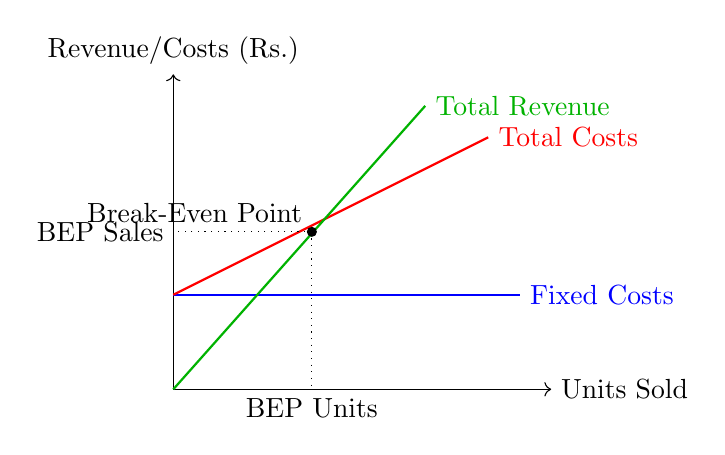
\begin{tikzpicture}[scale=0.8]
        \draw[->] (0,0) -- (6,0) node[right] {Units Sold};
        \draw[->] (0,0) -- (0,5) node[above] {Revenue/Costs (Rs.)};
        
        % Fixed Costs
        \draw[thick, blue] (0,1.5) -- (5.5,1.5) node[right] {Fixed Costs};
        
        % Total Costs
        \draw[thick, red] (0,1.5) -- (5,4) node[right] {Total Costs};
        
        % Total Revenue
        \draw[thick, green!70!black] (0,0) -- (4,4.5) node[right] {Total Revenue};
        
        % Break Even Point
        \filldraw[black] (2.2, 2.5) circle (2pt) node[above left] {Break-Even Point};
        
        % Dotted lines to axes
        \draw[dotted] (2.2, 2.5) -- (2.2, 0) node[below] {BEP Units};
        \draw[dotted] (2.2, 2.5) -- (0, 2.5) node[left] {BEP Sales};
        
    \end{tikzpicture}
    \captionof{figure}{Break-Even Chart}
\end{center}
\end{solutionbox}

\begin{mnemonicbox}
\mnemonic{"FCR" - Fixed Costs Contribution Ratio}
\end{mnemonicbox}

\questionmarks{2(c)}{7}{Explain the need of market survey and also explain the market test method of market survey.}

\begin{solutionbox}
\textbf{Answer}:

\textbf{Need of Market Survey:}

\begin{center}
\captionof{table}{Purpose of Market Survey}
\begin{tabulary}{\linewidth}{L L}
    \toprule
    \textbf{Purpose} & \textbf{Description} \\
    \midrule
    \textbf{Demand Assessment} & Understand customer needs and preferences \\
    \textbf{Competition Analysis} & Study competitor strategies and pricing \\
    \textbf{Market Size} & Estimate total addressable market \\
    \textbf{Pricing Strategy} & Determine optimal price points \\
    \bottomrule
\end{tabulary}
\end{center}

\textbf{Market Test Method:}

\begin{itemize}
    \item \keyword{Test Marketing}: Launch product in limited geographic area
    \item \keyword{Focus Groups}: Conduct discussions with target customers
    \item \keyword{Pilot Studies}: Small-scale product trials with selected customers
    \item \keyword{Online Surveys}: Digital questionnaires for broader reach
\end{itemize}

\begin{center}
    \begin{tikzpicture}[node distance=1.5cm, auto]
        \node [gtu block] (Need) {Market Survey Need};
        \node [gtu state, below left=of Need] (Demand) {Demand};
        \node [gtu state, below=of Need] (Comp) {Competition};
        \node [gtu state, below right=of Need] (Size) {Market Size};
        
        \node [gtu block, below=3cm of Need] (Method) {Market Test Methods};
        \node [gtu state, below left=of Method] (Test) {Test Marketing};
        \node [gtu state, below=of Method] (Focus) {Focus Groups};
        \node [gtu state, below right=of Method] (Pilot) {Pilot Studies};
        
        \draw [gtu arrow] (Need) -- (Demand);
        \draw [gtu arrow] (Need) -- (Comp);
        \draw [gtu arrow] (Need) -- (Size);
        
        \draw [gtu arrow] (Method) -- (Test);
        \draw [gtu arrow] (Method) -- (Focus);
        \draw [gtu arrow] (Method) -- (Pilot);
    \end{tikzpicture}
    \captionof{figure}{Market Survey Components}
\end{center}
\end{solutionbox}

\begin{mnemonicbox}
\mnemonic{"DCMP-TFPO" - Demand Competition Market Pricing Test Focus Pilot Online}
\end{mnemonicbox}

\questionmarks{2(a OR)}{3}{What is marketing plan? Explain in brief.}

\begin{solutionbox}
\textbf{Answer}:

A \textbf{marketing plan} is a strategic document outlining how a business will promote and sell its products or services to target customers.

\textbf{Components:}

\begin{itemize}
    \item \keyword{Market Analysis}: Customer demographics and behavior study
    \item \keyword{Marketing Mix}: Product, Price, Place, Promotion strategies
    \item \keyword{Budget Allocation}: Financial resources for marketing activities
\end{itemize}
\end{solutionbox}

\begin{mnemonicbox}
\mnemonic{"AMB" - Analysis Mix Budget}
\end{mnemonicbox}

\questionmarks{2(b OR)}{4}{Prepare SWOT analysis for a company manufacturing e-bike in urban region in Gujarat.}

\begin{solutionbox}
\textbf{Answer}:

\begin{center}
\captionof{table}{SWOT Analysis for E-bike Company}
\begin{tabulary}{\linewidth}{L L}
    \toprule
    \textbf{SWOT Analysis} & \textbf{E-bike Manufacturing Company} \\
    \midrule
    \textbf{Strengths} & $\bullet$ Government support for electric vehicles \newline $\bullet$ Growing environmental awareness \newline $\bullet$ Lower operating costs than petrol vehicles \\
    \textbf{Weaknesses} & $\bullet$ High initial investment \newline $\bullet$ Limited charging infrastructure \newline $\bullet$ Battery replacement costs \\
    \textbf{Opportunities} & $\bullet$ FAME scheme subsidies \newline $\bullet$ Urban pollution concerns \newline $\bullet$ Rising fuel prices \\
    \textbf{Threats} & $\bullet$ Competition from established players \newline $\bullet$ Technology obsolescence \newline $\bullet$ Economic slowdown affecting purchasing power \\
    \bottomrule
\end{tabulary}
\end{center}
\end{solutionbox}

\begin{mnemonicbox}
\mnemonic{"SWOT-GILH" - Strengths Weaknesses Opportunities Threats Government Infrastructure Low High}
\end{mnemonicbox}

\questionmarks{2(c OR)}{7}{What is innovation? List any five innovations of any product or process or service.}

\begin{solutionbox}
\textbf{Answer}:

\textbf{Innovation} is the process of creating new or improved products, services, or processes that provide value to customers and competitive advantage to organizations.

\textbf{Five Product/Service Innovations:}

\begin{center}
\captionof{table}{Examples of Innovation}
\begin{tabulary}{\linewidth}{L L L}
    \toprule
    \textbf{Innovation} & \textbf{Type} & \textbf{Description} \\
    \midrule
    \textbf{UPI Payment System} & Service & Digital payment platform revolutionizing transactions \\
    \textbf{Tesla Electric Cars} & Product & Sustainable automotive technology with autonomous features \\
    \textbf{Netflix Streaming} & Service & On-demand entertainment delivery model \\
    \textbf{3D Printing} & Process & Additive manufacturing technology \\
    \textbf{Zoom Video Calling} & Service & Remote communication platform for virtual meetings \\
    \bottomrule
\end{tabulary}
\end{center}

\begin{itemize}
    \item \keyword{Value Creation}: Each innovation solved existing customer problems
    \item \keyword{Market Disruption}: Changed traditional business models and user behavior
    \item \keyword{Technology Integration}: Combined multiple technologies for enhanced user experience
\end{itemize}
\end{solutionbox}

\begin{mnemonicbox}
\mnemonic{"UNTZI-VTM" - UPI Netflix Tesla Zoom Innovation Value Technology Market}
\end{mnemonicbox}

\questionmarks{3(a)}{3}{Write short note on partnership firm.}

\begin{solutionbox}
\textbf{Answer}:

A \textbf{partnership firm} is a business structure where two or more individuals jointly own and operate a business for profit.

\textbf{Key Features:}

\begin{itemize}
    \item \keyword{Shared Ownership}: Multiple partners contribute capital and expertise
    \item \keyword{Joint Liability}: Partners are personally liable for business debts
    \item \keyword{Profit Sharing}: Earnings distributed according to partnership agreement
\end{itemize}
\end{solutionbox}

\begin{mnemonicbox}
\mnemonic{"SJP" - Shared Joint Profit}
\end{mnemonicbox}

\questionmarks{3(b)}{4}{Explain the various activities involved in `staffing' function of management with example.}

\begin{solutionbox}
\textbf{Answer}:

\begin{center}
\captionof{table}{Staffing Activities}
\begin{tabulary}{\linewidth}{L L L}
    \toprule
    \textbf{Staffing Activity} & \textbf{Description} & \textbf{Example} \\
    \midrule
    \textbf{Recruitment} & Attracting potential candidates & Posting job advertisements on LinkedIn \\
    \textbf{Selection} & Choosing suitable candidates & Conducting interviews and aptitude tests \\
    \textbf{Training} & Skill development programs & New employee orientation sessions \\
    \textbf{Performance Appraisal} & Evaluating employee performance & Annual performance reviews \\
    \bottomrule
\end{tabulary}
\end{center}

\begin{itemize}
    \item \keyword{Placement}: Assigning right person to right job position
    \item \keyword{Promotion}: Career advancement based on performance and experience
    \item \keyword{Compensation}: Determining fair wages and benefits package
\end{itemize}
\end{solutionbox}

\begin{mnemonicbox}
\mnemonic{"RSTPPC" - Recruitment Selection Training Performance Placement Promotion Compensation}
\end{mnemonicbox}

\questionmarks{3(c)}{7}{Explain the autocratic leadership and state its advantages.}

\begin{solutionbox}
\textbf{Answer}:

\textbf{Autocratic Leadership} is a management style where the leader makes all decisions independently without consulting team members.

\textbf{Characteristics:}

\begin{itemize}
    \item \keyword{Centralized Decision Making}: Leader has complete authority and control
    \item \keyword{Clear Chain of Command}: Well-defined hierarchy and reporting structure
    \item \keyword{Limited Employee Input}: Minimal participation in decision-making process
\end{itemize}

\textbf{Advantages:}

\begin{center}
\captionof{table}{Advantages of Autocratic Leadership}
\begin{tabulary}{\linewidth}{L L}
    \toprule
    \textbf{Advantage} & \textbf{Description} \\
    \midrule
    \textbf{Quick Decisions} & Faster problem-solving without lengthy consultations \\
    \textbf{Clear Direction} & Employees know exactly what is expected \\
    \textbf{Crisis Management} & Effective during emergencies requiring immediate action \\
    \textbf{Productivity} & Higher output due to structured work environment \\
    \textbf{Accountability} & Single point of responsibility for outcomes \\
    \bottomrule
\end{tabulary}
\end{center}

\begin{center}
    \begin{tikzpicture}[node distance=1.5cm, auto]
        \node [gtu block] (Main) {Autocratic Leadership};
        \node [gtu state, below left=of Main] (Dec) {Centralized Decisions};
        \node [gtu state, below=of Main] (Cmd) {Clear Chain of Command};
        \node [gtu state, below right=of Main] (Inp) {Limited Input};
        
        \node [gtu block, below=3cm of Main] (Adv) {Advantages};
        \node [gtu state, below left=of Adv] (Quick) {Quick Decisions};
        \node [gtu state, below=of Adv] (Clear) {Clear Direction};
        \node [gtu state, below right=of Adv] (Prod) {Productivity};
        
        \draw [gtu arrow] (Main) -- (Dec);
        \draw [gtu arrow] (Main) -- (Cmd);
        \draw [gtu arrow] (Main) -- (Inp);
        
        \draw [gtu arrow] (Adv) -- (Quick);
        \draw [gtu arrow] (Adv) -- (Clear);
        \draw [gtu arrow] (Adv) -- (Prod);
    \end{tikzpicture}
    \captionof{figure}{Autocratic Leadership Model}
\end{center}
\end{solutionbox}

\begin{mnemonicbox}
\mnemonic{"QCCPA" - Quick Clear Crisis Productivity Accountability}
\end{mnemonicbox}


\questionmarks{3(a) OR}{3}{Write short note on joint stock company.}

\begin{solutionbox}
A \textbf{joint stock company} is a business organization where capital is divided into shares owned by multiple shareholders.

\textbf{Key Features:}
\begin{itemize}
    \item \textbf{Limited Liability}: Shareholders' liability limited to their investment
    \item \textbf{Transferable Shares}: Ownership can be easily bought and sold
    \item \textbf{Separate Legal Entity}: Company exists independently of its owners
\end{itemize}
\end{solutionbox}

\begin{mnemonicbox}
\mnemonic{"LTS" - Limited Transferable Separate}
\end{mnemonicbox}

\questionmarks{3(b) OR}{4}{Explain the various activities involved in 'organizing' function of management with example.}

\begin{solutionbox}
\begin{itemize}
    \item \textbf{Resource Allocation}: Distributing financial and human resources efficiently
    \item \textbf{Span of Control}: Determining number of subordinates per manager
    \item \textbf{Unity of Command}: Each employee reports to one superior
\end{itemize}

\begin{center}
\captionof{table}{Organizing Activities}
\begin{tabulary}{\linewidth}{|L|L|L|}
\hline
\textbf{Organizing Activity} & \textbf{Description} & \textbf{Example} \\ \hline
\textbf{Job Design} & Defining roles and responsibilities & Creating job descriptions for marketing manager \\ \hline
\textbf{Departmentalization} & Grouping similar activities & Forming HR, Finance, and Operations departments \\ \hline
\textbf{Delegation} & Assigning authority and responsibility & Manager delegating budget approval to team leads \\ \hline
\textbf{Coordination} & Ensuring smooth workflow & Weekly inter-department meetings \\ \hline
\end{tabulary}
\end{center}
\end{solutionbox}

\begin{mnemonicbox}
\mnemonic{"JDDCRSU" - Job Departmentalization Delegation Coordination Resource Span Unity}
\end{mnemonicbox}

\questionmarks{3(c) OR}{7}{Explain the democratic leadership and state its advantages.}

\begin{solutionbox}
\textbf{Democratic Leadership} is a management style where leaders involve team members in decision-making processes and encourage participation.

\textbf{Characteristics:}
\begin{itemize}
    \item \textbf{Participative Decision Making}: Team members contribute to problem-solving
    \item \textbf{Open Communication}: Two-way communication between leaders and employees
    \item \textbf{Shared Responsibility}: Collective ownership of outcomes and results
\end{itemize}

\textbf{Advantages:}
\begin{center}
\captionof{table}{Advantages of Democratic Leadership}
\begin{tabulary}{\linewidth}{|L|L|}
\hline
\textbf{Advantage} & \textbf{Description} \\ \hline
\textbf{Higher Job Satisfaction} & Employees feel valued and heard \\ \hline
\textbf{Better Quality Decisions} & Multiple perspectives improve decision quality \\ \hline
\textbf{Improved Creativity} & Diverse ideas and innovative solutions \\ \hline
\textbf{Team Building} & Stronger collaboration and trust \\ \hline
\textbf{Employee Development} & Skills enhancement through participation \\ \hline
\end{tabulary}
\end{center}

\begin{center}
\begin{tikzpicture}[node distance=1.5cm]
    \node [gtu block] (root) {Democratic Leadership};
    
    \node [gtu block, below left=1.2cm and 2cm of root] (char) {Characteristics};
    \node [gtu block, below right=1.2cm and 2cm of root] (adv) {Advantages};
    
    \node [gtu state, below=0.5cm of char, align=left] (c1) {Participative Decisions\\Open Communication\\Shared Responsibility};
    \node [gtu state, below=0.5cm of adv, align=left] (a1) {Job Satisfaction\\Quality Decisions\\Creativity\\Team Building};
    
    \draw [gtu arrow] (root) -- (char);
    \draw [gtu arrow] (root) -- (adv);
    \draw [gtu arrow] (char) -- (c1);
    \draw [gtu arrow] (adv) -- (a1);
\end{tikzpicture}
\captionof{figure}{Democratic Leadership Model}
\end{center}
\end{solutionbox}

\begin{mnemonicbox}
\mnemonic{"JQCTE" - Job Quality Creativity Team Employee}
\end{mnemonicbox}

\questionmarks{4(a)}{3}{State various functions of District Industries center.}

\begin{solutionbox}
\begin{itemize}
    \item \textbf{Registration Services}: MSME registration and various license approvals
    \item \textbf{Financial Assistance}: Guidance for loans and government scheme applications
    \item \textbf{Technical Support}: Providing technical guidance and consultancy services
\end{itemize}
\end{solutionbox}

\begin{mnemonicbox}
\mnemonic{"RFT" - Registration Financial Technical}
\end{mnemonicbox}

\questionmarks{4(b)}{4}{Identify any two state level incubators and write their functions.}

\begin{solutionbox}
\begin{center}
\captionof{table}{State Level Incubators}
\begin{tabulary}{\linewidth}{|L|L|}
\hline
\textbf{Incubator} & \textbf{Functions} \\ \hline
\textbf{i-HUB Gujarat} & \textbullet\ Startup mentoring and acceleration programs \\
& \textbullet\ Funding support and investor connections \\
& \textbullet\ Infrastructure and co-working space facilities \\ \hline
\textbf{CIIE Ahmedabad} & \textbullet\ Technology commercialization support \\
& \textbullet\ Industry-academia collaboration \\
& \textbullet\ Scale-up programs for growing startups \\ \hline
\end{tabulary}
\end{center}

\textbf{Common Functions:}
\begin{itemize}
    \item \textbf{Mentorship Programs}: Expert guidance from industry professionals
    \item \textbf{Networking Events}: Connecting startups with investors and partners
\end{itemize}
\end{solutionbox}

\begin{mnemonicbox}
\mnemonic{"MFIN" - Mentoring Funding Infrastructure Networking}
\end{mnemonicbox}

\questionmarks{4(c)}{7}{What is start-up eco system? List various activities and elements of start-up eco system.}

\begin{solutionbox}
\textbf{Start-up Ecosystem} is a interconnected network of organizations, individuals, and resources that support entrepreneurship and startup development.

\textbf{Key Elements:}
\begin{center}
\captionof{table}{Startup Ecosystem Elements}
\begin{tabulary}{\linewidth}{|L|L|}
\hline
\textbf{Element} & \textbf{Description} \\ \hline
\textbf{Entrepreneurs} & Visionary individuals starting new ventures \\ \hline
\textbf{Investors} & Angel investors, VCs providing funding \\ \hline
\textbf{Incubators/Accelerators} & Support organizations for early-stage startups \\ \hline
\textbf{Government} & Policy makers and regulatory bodies \\ \hline
\textbf{Educational Institutions} & Universities and research centers \\ \hline
\textbf{Service Providers} & Legal, accounting, consulting firms \\ \hline
\end{tabulary}
\end{center}

\textbf{Activities:}
\begin{itemize}
    \item \textbf{Mentoring Sessions}: Regular guidance from experienced entrepreneurs
    \item \textbf{Networking Events}: Startup meetups and investor pitch sessions
    \item \textbf{Funding Rounds}: Seed, Series A, B funding opportunities
    \item \textbf{Skill Development}: Technical and business training programs
\end{itemize}

\begin{center}
\begin{tikzpicture}[node distance=1.5cm]
    \node [gtu block] (root) {Start-up Ecosystem};
    
    \node [gtu block, below left=1.2cm and 2.5cm of root] (elem) {Key Elements};
    \node [gtu block, below right=1.2cm and 2.5cm of root] (act) {Activities};
    
    \node [gtu state, below=0.5cm of elem, align=left] (e1) {Entrepreneurs\\Investors\\Incubators\\Government\\Education\\Service Providers};
    \node [gtu state, below=0.5cm of act, align=left] (a1) {Mentoring Sessions\\Networking Events\\Funding Rounds\\Skill Development};
    
    \draw [gtu arrow] (root) -- (elem);
    \draw [gtu arrow] (root) -- (act);
    \draw [gtu arrow] (elem) -- (e1);
    \draw [gtu arrow] (act) -- (a1);
\end{tikzpicture}
\captionof{figure}{Ecosystem Components}
\end{center}
\end{solutionbox}

\begin{mnemonicbox}
\mnemonic{"EIGEES-MNFS" - Entrepreneurs Investors Government Education Service Mentoring Networking Funding Skill}
\end{mnemonicbox}

\questionmarks{4(a) OR}{3}{State various functions of Small industries Development Bank of India (SIDBI).}

\begin{solutionbox}
\begin{itemize}
    \item \textbf{Financial Services}: Direct and indirect lending to MSMEs and startups
    \item \textbf{Development Services}: Capacity building and skill development programs
    \item \textbf{Promotional Activities}: Market development and technology upgradation support
\end{itemize}
\end{solutionbox}

\begin{mnemonicbox}
\mnemonic{"FDP" - Financial Development Promotional}
\end{mnemonicbox}

\questionmarks{4(b) OR}{4}{Identify any two national level incubators and write their functions.}

\begin{solutionbox}
\begin{center}
\captionof{table}{National Level Incubators}
\begin{tabulary}{\linewidth}{|L|L|}
\hline
\textbf{Incubator} & \textbf{Functions} \\ \hline
\textbf{T-Hub Hyderabad} & \textbullet\ India's largest startup incubator \\
& \textbullet\ Technology innovation and R\&D support \\
& \textbullet\ Global market access programs \\ \hline
\textbf{NASSCOM 10,000 Startups} & \textbullet\ Pan-India startup acceleration program \\
& \textbullet\ Corporate partnership facilitation \\
& \textbullet\ Ecosystem building and policy advocacy \\ \hline
\end{tabulary}
\end{center}

\textbf{Common Functions:}
\begin{itemize}
    \item \textbf{Acceleration Programs}: Intensive startup development and mentoring
    \item \textbf{Corporate Connections}: Linking startups with large enterprise partners
\end{itemize}
\end{solutionbox}

\begin{mnemonicbox}
\mnemonic{"TIGAC" - Technology Innovation Global Acceleration Corporate}
\end{mnemonicbox}

\questionmarks{4(c) OR}{7}{Which steps should be taken to avoid failure of start-up? Explain in brief.}

\begin{solutionbox}
\textbf{Steps to Avoid Startup Failure:}

\begin{center}
\captionof{table}{Strategies for Success}
\begin{tabulary}{\linewidth}{|L|L|}
\hline
\textbf{Step} & \textbf{Description} \\ \hline
\textbf{Market Research} & Thorough understanding of customer needs and market demand \\ \hline
\textbf{Financial Planning} & Proper cash flow management and funding strategies \\ \hline
\textbf{Team Building} & Hiring skilled and committed team members \\ \hline
\textbf{Product Validation} & Testing product-market fit before full launch \\ \hline
\textbf{Customer Focus} & Continuous customer feedback and satisfaction \\ \hline
\end{tabulary}
\end{center}

\textbf{Additional Measures:}
\begin{itemize}
    \item \textbf{Risk Management}: Identifying potential threats and mitigation strategies
    \item \textbf{Adaptability}: Flexibility to pivot based on market changes
    \item \textbf{Legal Compliance}: Proper registration and regulatory adherence
\end{itemize}

\begin{center}
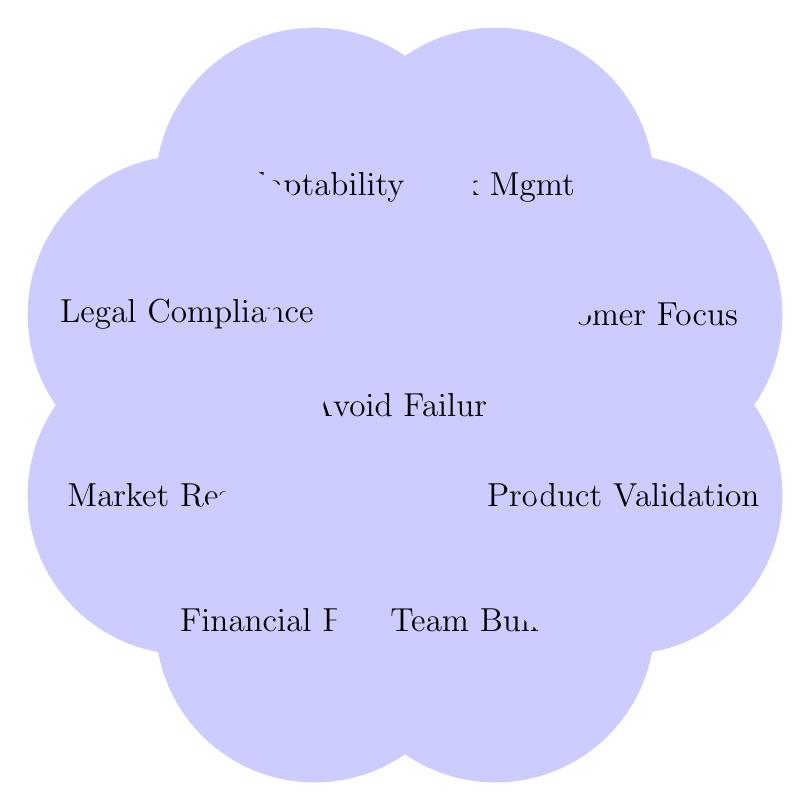
\begin{tikzpicture}[mindmap, grow cyclic, every node/.style=concept, concept color=blue!20,
    level 1/.style={level distance=3cm, sibling angle=45},
    level 2/.style={level distance=3cm, sibling angle=45}]
    
    \node [concept] {Avoid Failure}
    child { node [concept] {Market Research} }
    child { node [concept] {Financial Planning} }
    child { node [concept] {Team Building} }
    child { node [concept] {Product Validation} }
    child { node [concept] {Customer Focus} }
    child { node [concept] {Risk Mgmt} }
    child { node [concept] {Adaptability} }
    child { node [concept] {Legal Compliance} };
\end{tikzpicture}
\captionof{figure}{Startup Success Strategies}
\end{center}
\end{solutionbox}

\begin{mnemonicbox}
\mnemonic{"MFTPCRAL" - Market Financial Team Product Customer Risk Adaptability Legal}
\end{mnemonicbox}

\questionmarks{5(a)}{3}{How Return on Investment (ROI) is calculated?}

\begin{solutionbox}
\textbf{ROI Formula:}
\[ \text{ROI} = \left( \frac{\text{Net Profit}}{\text{Total Investment}} \right) \times 100 \]

\textbf{Example:}
\begin{itemize}
    \item Investment = Rs. 1,00,000
    \item Net Profit = Rs. 20,000
    \item ROI = $(20,000 / 1,00,000) \times 100 = 20\%$
\end{itemize}
\end{solutionbox}

\begin{mnemonicbox}
\mnemonic{"NTH" - Net Total Hundred}
\end{mnemonicbox}

\questionmarks{5(b)}{4}{Show the significance of technical analysis in feasibility study.}

\begin{solutionbox}
\begin{center}
\captionof{table}{Significance of Technical Analysis}
\begin{tabulary}{\linewidth}{|L|L|}
\hline
\textbf{Significance} & \textbf{Description} \\ \hline
\textbf{Technology Assessment} & Evaluating technical viability and requirements \\ \hline
\textbf{Resource Planning} & Determining machinery, equipment, and infrastructure needs \\ \hline
\textbf{Process Design} & Optimal production methods and workflow \\ \hline
\textbf{Quality Standards} & Ensuring product meets industry specifications \\ \hline
\end{tabulary}
\end{center}
\end{solutionbox}

\begin{mnemonicbox}
\mnemonic{"TRPQ" - Technology Resource Process Quality}
\end{mnemonicbox}

\questionmarks{5(c)}{7}{Explain the characteristics of corporate social responsibility.}

\begin{solutionbox}
\textbf{Corporate Social Responsibility (CSR)} refers to business practices involving initiatives that benefit society and demonstrate commitment to ethical operations.

\textbf{Key Characteristics:}
\begin{center}
\captionof{table}{CSR Characteristics}
\begin{tabulary}{\linewidth}{|L|L|}
\hline
\textbf{Characteristic} & \textbf{Description} \\ \hline
\textbf{Voluntary Nature} & Beyond legal requirements, self-imposed commitments \\ \hline
\textbf{Stakeholder Orientation} & Considering impact on all stakeholders, not just shareholders \\ \hline
\textbf{Triple Bottom Line} & Focus on People, Planet, and Profit \\ \hline
\textbf{Sustainable Practices} & Long-term environmental and social sustainability \\ \hline
\textbf{Transparency} & Open reporting and accountability \\ \hline
\end{tabulary}
\end{center}

\textbf{CSR Areas:}
\begin{itemize}
    \item \textbf{Community Development}: Education, healthcare, and infrastructure projects
    \item \textbf{Environmental Protection}: Pollution control and resource conservation
    \item \textbf{Employee Welfare}: Fair wages, safe working conditions, skill development
\end{itemize}

\begin{center}
\begin{tikzpicture}[node distance=1.5cm]
    \node [gtu block] (root) {CSR};
    
    \node [gtu block, below left=1.2cm and 2cm of root] (char) {Characteristics};
    \node [gtu block, below right=1.2cm and 2cm of root] (act) {Activities};
    
    \node [gtu state, below=0.5cm of char, align=left] (c1) {Voluntary\\Stakeholder Focus\\Triple Bottom Line\\Sustainability};
    \node [gtu state, below=0.5cm of act, align=left] (a1) {Community Dev\\Environment\\Employee Welfare};
    
    \draw [gtu arrow] (root) -- (char);
    \draw [gtu arrow] (root) -- (act);
    \draw [gtu arrow] (char) -- (c1);
    \draw [gtu arrow] (act) -- (a1);
\end{tikzpicture}
\captionof{figure}{CSR Framework}
\end{center}
\end{solutionbox}

\begin{mnemonicbox}
\mnemonic{"VSTST-CEE" - Voluntary Stakeholder Triple Sustainable Transparency Community Environmental Employee}
\end{mnemonicbox}

\questionmarks{5(a) OR}{3}{How Return on Sales (ROS) is calculated?}

\begin{solutionbox}
\textbf{ROS Formula:}
\[ \text{ROS} = \left( \frac{\text{Net Profit}}{\text{Net Sales}} \right) \times 100 \]

\textbf{Example:}
\begin{itemize}
    \item Net Sales = Rs. 5,00,000
    \item Net Profit = Rs. 50,000
    \item ROS = $(50,000 / 5,00,000) \times 100 = 10\%$
\end{itemize}
\end{solutionbox}

\begin{mnemonicbox}
\mnemonic{"NSH" - Net Sales Hundred}
\end{mnemonicbox}

\questionmarks{5(b) OR}{4}{Show the significance of market analysis in feasibility study.}

\begin{solutionbox}
\begin{center}
\captionof{table}{Significance of Market Analysis}
\begin{tabulary}{\linewidth}{|L|L|}
\hline
\textbf{Significance} & \textbf{Description} \\ \hline
\textbf{Demand Forecasting} & Estimating future market size and growth \\ \hline
\textbf{Competition Assessment} & Understanding competitive landscape \\ \hline
\textbf{Pricing Strategy} & Determining optimal price points \\ \hline
\textbf{Market Segmentation} & Identifying target customer groups \\ \hline
\end{tabulary}
\end{center}
\end{solutionbox}

\begin{mnemonicbox}
\mnemonic{"DCPM" - Demand Competition Pricing Market}
\end{mnemonicbox}

\questionmarks{5(c) OR}{7}{Explain the characteristics of ethics.}

\begin{solutionbox}
\textbf{Ethics} are moral principles that govern behavior and decision-making in personal and professional contexts.

\textbf{Key Characteristics:}
\begin{center}
\captionof{table}{Characteristics of Ethics}
\begin{tabulary}{\linewidth}{|L|L|}
\hline
\textbf{Characteristic} & \textbf{Description} \\ \hline
\textbf{Universal Principles} & Apply across cultures and situations \\ \hline
\textbf{Moral Standards} & Based on concepts of right and wrong \\ \hline
\textbf{Voluntary Compliance} & Internal motivation rather than external force \\ \hline
\textbf{Consequential Thinking} & Considering outcomes and impacts \\ \hline
\textbf{Stakeholder Consideration} & Accounting for all affected parties \\ \hline
\end{tabulary}
\end{center}

\textbf{Core Values:}
\begin{itemize}
    \item \textbf{Consistency}: Ethical behavior remains constant across situations
    \item \textbf{Transparency}: Open and honest communication and actions
    \item \textbf{Accountability}: Taking responsibility for decisions and their consequences
\end{itemize}

\begin{center}
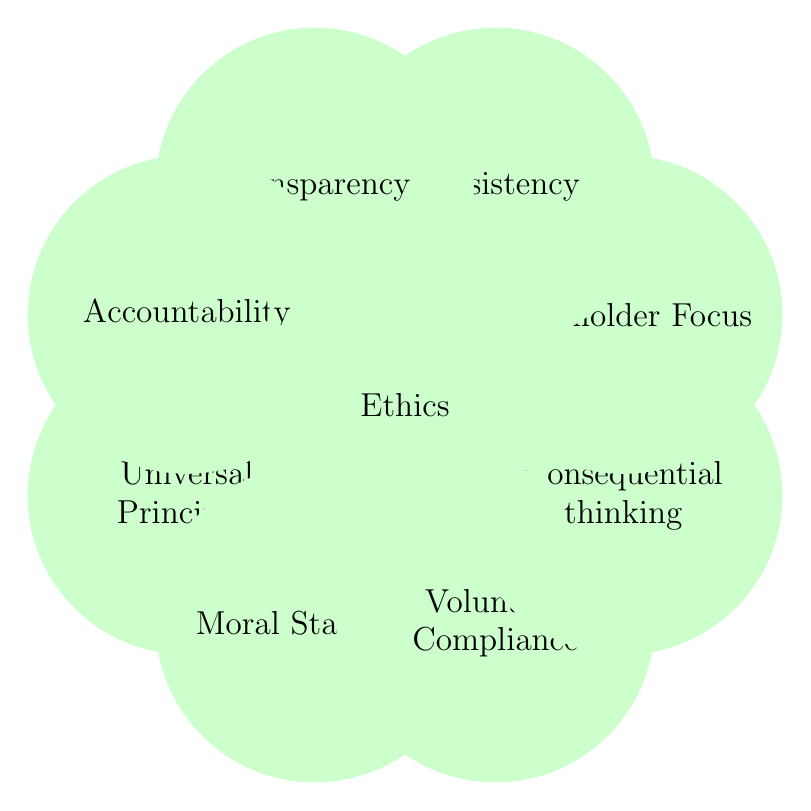
\begin{tikzpicture}[mindmap, grow cyclic, every node/.style=concept, concept color=green!20,
    level 1/.style={level distance=3cm, sibling angle=45}]
    
    \node [concept] {Ethics}
    child { node [concept] {Universal Principles} }
    child { node [concept] {Moral Standards} }
    child { node [concept] {Voluntary Compliance} }
    child { node [concept] {Consequential thinking} }
    child { node [concept] {Stakeholder Focus} }
    child { node [concept] {Consistency} }
    child { node [concept] {Transparency} }
    child { node [concept] {Accountability} };
\end{tikzpicture}
\captionof{figure}{Key Ethical Characteristics}
\end{center}
\end{solutionbox}

\begin{mnemonicbox}
\mnemonic{"UMVCSCTA" - Universal Moral Voluntary Consequential Stakeholder Consistency Transparency Accountability}
\end{mnemonicbox}

\end{document}

\questionmarks{3(a OR)}{3}{Write short note on joint stock company.}

\begin{solutionbox}
\textbf{Answer}:

A \textbf{joint stock company} is a business organization where capital is divided into shares owned by multiple shareholders.

\textbf{Key Features:}

\begin{itemize}
    \item \keyword{Limited Liability}: Shareholders' liability limited to their investment
    \item \keyword{Transferable Shares}: Ownership can be easily bought and sold
    \item \keyword{Separate Legal Entity}: Company exists independently of its owners
\end{itemize}
\end{solutionbox}

\begin{mnemonicbox}
\mnemonic{"LTS" - Limited Transferable Separate}
\end{mnemonicbox}

\questionmarks{3(b OR)}{4}{Explain the various activities involved in `organizing' function of management with example.}

\begin{solutionbox}
\textbf{Answer}:

\begin{center}
\captionof{table}{Organizing Activities}
\begin{tabulary}{\linewidth}{L L L}
    \toprule
    \textbf{Organizing Activity} & \textbf{Description} & \textbf{Example} \\
    \midrule
    \textbf{Job Design} & Defining roles and responsibilities & Creating job descriptions for marketing manager \\
    \textbf{Departmentalization} & Grouping similar activities & Forming HR, Finance, and Operations departments \\
    \textbf{Delegation} & Assigning authority and responsibility & Manager delegating budget approval to team leads \\
    \textbf{Coordination} & Ensuring smooth workflow & Weekly inter-department meetings \\
    \bottomrule
\end{tabulary}
\end{center}

\begin{itemize}
    \item \keyword{Resource Allocation}: Distributing financial and human resources efficiently
    \item \keyword{Span of Control}: Determining number of subordinates per manager
    \item \keyword{Unity of Command}: Each employee reports to one superior
\end{itemize}
\end{solutionbox}

\begin{mnemonicbox}
\mnemonic{"JDDCRSU" - Job Departmentalization Delegation Coordination Resource Span Unity}
\end{mnemonicbox}

\questionmarks{3(c OR)}{7}{Explain the democratic leadership and state its advantages.}

\begin{solutionbox}
\textbf{Answer}:

\textbf{Democratic Leadership} is a management style where leaders involve team members in decision-making processes and encourage participation.

\textbf{Characteristics:}

\begin{itemize}
    \item \keyword{Participative Decision Making}: Team members contribute to problem-solving
    \item \keyword{Open Communication}: Two-way communication between leaders and employees
    \item \keyword{Shared Responsibility}: Collective ownership of outcomes and results
\end{itemize}

\textbf{Advantages:}

\begin{center}
\captionof{table}{Advantages of Democratic Leadership}
\begin{tabulary}{\linewidth}{L L}
    \toprule
    \textbf{Advantage} & \textbf{Description} \\
    \midrule
    \textbf{Higher Job Satisfaction} & Employees feel valued and heard \\
    \textbf{Better Quality Decisions} & Multiple perspectives improve decision quality \\
    \textbf{Improved Creativity} & Diverse ideas and innovative solutions \\
    \textbf{Team Building} & Stronger collaboration and trust \\
    \textbf{Employee Development} & Skills enhancement through participation \\
    \bottomrule
\end{tabulary}
\end{center}

\begin{center}
    \begin{tikzpicture}[node distance=1.5cm, auto]
        \node [gtu block] (Main) {Democratic Leadership};
        \node [gtu state, below left=of Main] (Part) {Participative Decisions};
        \node [gtu state, below=of Main] (Comm) {Open Communication};
        \node [gtu state, below right=of Main] (Resp) {Shared Responsibility};

        \node [gtu block, below=3cm of Main] (Adv) {Advantages};
        \node [gtu state, below left=of Adv] (Sat) {Job Satisfaction};
        \node [gtu state, below=of Adv] (Qual) {Quality Decisions};
        \node [gtu state, below right=of Adv] (Creat) {Creativity};

        \draw [gtu arrow] (Main) -- (Part);
        \draw [gtu arrow] (Main) -- (Comm);
        \draw [gtu arrow] (Main) -- (Resp);

        \draw [gtu arrow] (Adv) -- (Sat);
        \draw [gtu arrow] (Adv) -- (Qual);
        \draw [gtu arrow] (Adv) -- (Creat);
    \end{tikzpicture}
    \captionof{figure}{Democratic Leadership Model}
\end{center}
\end{solutionbox}

\begin{mnemonicbox}
\mnemonic{"JQCTE" - Job Quality Creativity Team Employee}
\end{mnemonicbox}

\questionmarks{4(a)}{3}{State various functions of District Industries center.}

\begin{solutionbox}
\textbf{Answer}:

\begin{itemize}
    \item \keyword{Registration Services}: MSME registration and various license approvals
    \item \keyword{Financial Assistance}: Guidance for loans and government scheme applications
    \item \keyword{Technical Support}: Providing technical guidance and consultancy services
\end{itemize}
\end{solutionbox}

\begin{mnemonicbox}
\mnemonic{"RFT" - Registration Financial Technical}
\end{mnemonicbox}

\questionmarks{4(b)}{4}{Identify any two state level incubators and write their functions.}

\begin{solutionbox}
\textbf{Answer}:

\begin{center}
\captionof{table}{State Level Incubators}
\begin{tabulary}{\linewidth}{L L}
    \toprule
    \textbf{Incubator} & \textbf{Functions} \\
    \midrule
    \textbf{i-HUB Gujarat} & $\bullet$ Startup mentoring and acceleration programs \newline $\bullet$ Funding support and investor connections \newline $\bullet$ Infrastructure and co-working space facilities \\
    \textbf{CIIE Ahmedabad} & $\bullet$ Technology commercialization support \newline $\bullet$ Industry-academia collaboration \newline $\bullet$ Scale-up programs for growing startups \\
    \bottomrule
\end{tabulary}
\end{center}

\textbf{Common Functions:}

\begin{itemize}
    \item \keyword{Mentorship Programs}: Expert guidance from industry professionals
    \item \keyword{Networking Events}: Connecting startups with investors and partners
\end{itemize}
\end{solutionbox}

\begin{mnemonicbox}
\mnemonic{"MFIN" - Mentoring Funding Infrastructure Networking}
\end{mnemonicbox}

\questionmarks{4(c)}{7}{What is start-up eco system? List various activities and elements of start-up eco system.}

\begin{solutionbox}
\textbf{Answer}:

\textbf{Start-up Ecosystem} is a interconnected network of organizations, individuals, and resources that support entrepreneurship and startup development.

\textbf{Key Elements:}

\begin{center}
\captionof{table}{Startup Ecosystem Elements}
\begin{tabulary}{\linewidth}{L L}
    \toprule
    \textbf{Element} & \textbf{Description} \\
    \midrule
    \textbf{Entrepreneurs} & Visionary individuals starting new ventures \\
    \textbf{Investors} & Angel investors, VCs providing funding \\
    \textbf{Incubators/Accelerators} & Support organizations for early-stage startups \\
    \textbf{Government} & Policy makers and regulatory bodies \\
    \textbf{Educational Institutions} & Universities and research centers \\
    \textbf{Service Providers} & Legal, accounting, consulting firms \\
    \bottomrule
\end{tabulary}
\end{center}

\textbf{Activities:}

\begin{itemize}
    \item \keyword{Mentoring Sessions}: Regular guidance from experienced entrepreneurs
    \item \keyword{Networking Events}: Startup meetups and investor pitch sessions
    \item \keyword{Funding Rounds}: Seed, Series A, B funding opportunities
    \item \keyword{Skill Development}: Technical and business training programs
\end{itemize}

\begin{center}
    \begin{tikzpicture}[node distance=1.5cm, auto]
        \node [gtu block] (Main) {Startup Ecosystem};
        
        \node [gtu state, above=of Main] (Gov) {Government};
        \node [gtu state, below=of Main] (Inv) {Investors};
        \node [gtu state, left=of Main] (Ent) {Entrepreneurs};
        \node [gtu state, right=of Main] (Inc) {Incubators};
        \node [gtu state, above left=of Main] (Edu) {Education};
        \node [gtu state, below right=of Main] (Serv) {Services};

        \draw [gtu arrow] (Main) -- (Gov);
        \draw [gtu arrow] (Main) -- (Inv);
        \draw [gtu arrow] (Main) -- (Ent);
        \draw [gtu arrow] (Main) -- (Inc);
        \draw [gtu arrow] (Main) -- (Edu);
        \draw [gtu arrow] (Main) -- (Serv);
    \end{tikzpicture}
    \captionof{figure}{Startup Ecosystem Structure}
\end{center}
\end{solutionbox}

\begin{mnemonicbox}
\mnemonic{"EIGEES-MNFS" - Entrepreneurs Investors Government Education Service Mentoring Networking Funding Skill}
\end{mnemonicbox}

\questionmarks{4(a OR)}{3}{State various functions of Small industries Development Bank of India (SIDBI).}

\begin{solutionbox}
\textbf{Answer}:

\begin{itemize}
    \item \keyword{Financial Services}: Direct and indirect lending to MSMEs and startups
    \item \keyword{Development Services}: Capacity building and skill development programs
    \item \keyword{Promotional Activities}: Market development and technology upgradation support
\end{itemize}
\end{solutionbox}

\begin{mnemonicbox}
\mnemonic{"FDP" - Financial Development Promotional}
\end{mnemonicbox}

\questionmarks{4(b OR)}{4}{Identify any two national level incubators and write their functions.}

\begin{solutionbox}
\textbf{Answer}:

\begin{center}
\captionof{table}{National Level Incubators}
\begin{tabulary}{\linewidth}{L L}
    \toprule
    \textbf{Incubator} & \textbf{Functions} \\
    \midrule
    \textbf{T-Hub Hyderabad} & $\bullet$ India's largest startup incubator \newline $\bullet$ Technology innovation and R&D support \newline $\bullet$ Global market access programs \\
    \textbf{NASSCOM 10,000 Startups} & $\bullet$ Pan-India startup acceleration program \newline $\bullet$ Corporate partnership facilitation \newline $\bullet$ Ecosystem building and policy advocacy \\
    \bottomrule
\end{tabulary}
\end{center}

\textbf{Common Functions:}

\begin{itemize}
    \item \keyword{Acceleration Programs}: Intensive startup development and mentoring
    \item \keyword{Corporate Connections}: Linking startups with large enterprise partners
\end{itemize}
\end{solutionbox}

\begin{mnemonicbox}
\mnemonic{"TIGAC" - Technology Innovation Global Acceleration Corporate}
\end{mnemonicbox}

\questionmarks{4(c OR)}{7}{Which steps should be taken to avoid failure of start-up? Explain in brief.}

\begin{solutionbox}
\textbf{Answer}:

\textbf{Steps to Avoid Startup Failure:}

\begin{center}
\captionof{table}{Avoid Startup Failure}
\begin{tabulary}{\linewidth}{L L}
    \toprule
    \textbf{Step} & \textbf{Description} \\
    \midrule
    \textbf{Market Research} & Thorough understanding of customer needs and market demand \\
    \textbf{Financial Planning} & Proper cash flow management and funding strategies \\
    \textbf{Team Building} & Hiring skilled and committed team members \\
    \textbf{Product Validation} & Testing product-market fit before full launch \\
    \textbf{Customer Focus} & Continuous customer feedback and satisfaction \\
    \bottomrule
\end{tabulary}
\end{center}

\begin{itemize}
    \item \keyword{Risk Management}: Identifying potential threats and mitigation strategies
    \item \keyword{Adaptability}: Flexibility to pivot based on market changes
    \item \keyword{Legal Compliance}: Proper registration and regulatory adherence
\end{itemize}

\begin{center}
    \begin{tikzpicture}[node distance=1.5cm, auto]
        \node [gtu block] (Main) {Avoid Startup Failure};
        \node [gtu state, below left=of Main] (Mark) {Market Research};
        \node [gtu state, below=of Main] (Fin) {Financial Planning};
        \node [gtu state, below right=of Main] (Team) {Team Building};
        \node [gtu state, left=of Main] (Prod) {Product Validation};
        \node [gtu state, right=of Main] (Cust) {Customer Focus};

        \draw [gtu arrow] (Main) -- (Mark);
        \draw [gtu arrow] (Main) -- (Fin);
        \draw [gtu arrow] (Main) -- (Team);
        \draw [gtu arrow] (Main) -- (Prod);
        \draw [gtu arrow] (Main) -- (Cust);
    \end{tikzpicture}
    \captionof{figure}{Key Steps to Avoid Failure}
\end{center}
\end{solutionbox}

\begin{mnemonicbox}
\mnemonic{"MFTPCRAL" - Market Financial Team Product Customer Risk Adaptability Legal}
\end{mnemonicbox}

\questionmarks{5(a)}{3}{How Return on Investment (ROI) is calculated?}

\begin{solutionbox}
\textbf{Answer}:

\textbf{ROI Formula:} ROI = (Net Profit $\div$ Total Investment) $\times$ 100

\textbf{Example:}

\begin{itemize}
    \item Investment = ₹1,00,000
    \item Net Profit = ₹20,000
    \item ROI = (20,000 $\div$ 1,00,000) $\times$ 100 = 20\%
\end{itemize}
\end{solutionbox}

\begin{mnemonicbox}
\mnemonic{"NTH" - Net Total Hundred}
\end{mnemonicbox}

\questionmarks{5(b)}{4}{Show the significance of technical analysis in feasibility study.}

\begin{solutionbox}
\textbf{Answer}:

\begin{center}
\captionof{table}{Technical Analysis Significance}
\begin{tabulary}{\linewidth}{L L}
    \toprule
    \textbf{Significance} & \textbf{Description} \\
    \midrule
    \textbf{Technology Assessment} & Evaluating technical viability and requirements \\
    \textbf{Resource Planning} & Determining machinery, equipment, and infrastructure needs \\
    \textbf{Process Design} & Optimal production methods and workflow \\
    \textbf{Quality Standards} & Ensuring product meets industry specifications \\
    \bottomrule
\end{tabulary}
\end{center}
\end{solutionbox}

\begin{mnemonicbox}
\mnemonic{"TRPQ" - Technology Resource Process Quality}
\end{mnemonicbox}

\questionmarks{5(c)}{7}{Explain the characteristics of corporate social responsibility.}

\begin{solutionbox}
\textbf{Answer}:

\textbf{Corporate Social Responsibility (CSR)} refers to business practices involving initiatives that benefit society and demonstrate commitment to ethical operations.

\textbf{Key Characteristics:}

\begin{center}
\captionof{table}{CSR Characteristics}
\begin{tabulary}{\linewidth}{L L}
    \toprule
    \textbf{Characteristic} & \textbf{Description} \\
    \midrule
    \textbf{Voluntary Nature} & Beyond legal requirements, self-imposed commitments \\
    \textbf{Stakeholder Orientation} & Considering impact on all stakeholders, not just shareholders \\
    \textbf{Triple Bottom Line} & Focus on People, Planet, and Profit \\
    \textbf{Sustainable Practices} & Long-term environmental and social sustainability \\
    \textbf{Transparency} & Open reporting and accountability \\
    \bottomrule
\end{tabulary}
\end{center}

\begin{itemize}
    \item \keyword{Community Development}: Education, healthcare, and infrastructure projects
    \item \keyword{Environmental Protection}: Pollution control and resource conservation
    \item \keyword{Employee Welfare}: Fair wages, safe working conditions, skill development
\end{itemize}

\begin{center}
    \begin{tikzpicture}[node distance=1.5cm, auto]
        \node [gtu block] (Main) {CSR Characteristics};
        \node [gtu state, below left=of Main] (Vol) {Voluntary};
        \node [gtu state, below=of Main] (Stake) {Stakeholder};
        \node [gtu state, below right=of Main] (Trip) {Triple Bottom Line};
        
        \node [gtu block, below=3cm of Main] (Act) {CSR Activities};
        \node [gtu state, below left=of Act] (Comm) {Community};
        \node [gtu state, below=of Act] (Env) {Environment};
        \node [gtu state, below right=of Act] (Emp) {Employee};

        \draw [gtu arrow] (Main) -- (Vol);
        \draw [gtu arrow] (Main) -- (Stake);
        \draw [gtu arrow] (Main) -- (Trip);
        
        \draw [gtu arrow] (Act) -- (Comm);
        \draw [gtu arrow] (Act) -- (Env);
        \draw [gtu arrow] (Act) -- (Emp);
    \end{tikzpicture}
    \captionof{figure}{CSR Overview}
\end{center}
\end{solutionbox}

\begin{mnemonicbox}
\mnemonic{"VSTST-CEE" - Voluntary Stakeholder Triple Sustainable Transparency Community Environmental Employee}
\end{mnemonicbox}

\questionmarks{5(a OR)}{3}{How Return on Sales (ROS) is calculated?}

\begin{solutionbox}
\textbf{Answer}:

\textbf{ROS Formula:} ROS = (Net Profit $\div$ Net Sales) $\times$ 100

\textbf{Example:}

\begin{itemize}
    \item Net Sales = ₹5,00,000
    \item Net Profit = ₹50,000
    \item ROS = (50,000 $\div$ 5,00,000) $\times$ 100 = 10\%
\end{itemize}
\end{solutionbox}

\begin{mnemonicbox}
\mnemonic{"NSH" - Net Sales Hundred}
\end{mnemonicbox}

\questionmarks{5(b OR)}{4}{Show the significance of market analysis in feasibility study.}

\begin{solutionbox}
\textbf{Answer}:

\begin{center}
\captionof{table}{Market Analysis Significance}
\begin{tabulary}{\linewidth}{L L}
    \toprule
    \textbf{Significance} & \textbf{Description} \\
    \midrule
    \textbf{Demand Forecasting} & Estimating future market size and growth \\
    \textbf{Competition Assessment} & Understanding competitive landscape \\
    \textbf{Pricing Strategy} & Determining optimal price points \\
    \textbf{Market Segmentation} & Identifying target customer groups \\
    \bottomrule
\end{tabulary}
\end{center}
\end{solutionbox}

\begin{mnemonicbox}
\mnemonic{"DCPM" - Demand Competition Pricing Market}
\end{mnemonicbox}

\questionmarks{5(c OR)}{7}{Explain the characteristics of ethics.}

\begin{solutionbox}
\textbf{Answer}:

\textbf{Ethics} are moral principles that govern behavior and decision-making in personal and professional contexts.

\textbf{Key Characteristics:}

\begin{center}
\captionof{table}{Ethics Characteristics}
\begin{tabulary}{\linewidth}{L L}
    \toprule
    \textbf{Characteristic} & \textbf{Description} \\
    \midrule
    \textbf{Universal Principles} & Apply across cultures and situations \\
    \textbf{Moral Standards} & Based on concepts of right and wrong \\
    \textbf{Voluntary Compliance} & Internal motivation rather than external force \\
    \textbf{Consequential Thinking} & Considering outcomes and impacts \\
    \textbf{Stakeholder Consideration} & Accounting for all affected parties \\
    \bottomrule
\end{tabulary}
\end{center}

\begin{itemize}
    \item \keyword{Consistency}: Ethical behavior remains constant across situations
    \item \keyword{Transparency}: Open and honest communication and actions
    \item \keyword{Accountability}: Taking responsibility for decisions and their consequences
\end{itemize}

\begin{center}
    \begin{tikzpicture}[node distance=1.5cm, auto]
        \node [gtu block] (Main) {Ethics Characteristics};
        \node [gtu state, below left=of Main] (Univ) {Universal Principles};
        \node [gtu state, below=of Main] (Moral) {Moral Standards};
        \node [gtu state, below right=of Main] (Vol) {Voluntary};
        
        \node [gtu state, left=of Main] (Cons) {Consistency};
        \node [gtu state, right=of Main] (Trans) {Transparency};

        \draw [gtu arrow] (Main) -- (Univ);
        \draw [gtu arrow] (Main) -- (Moral);
        \draw [gtu arrow] (Main) -- (Vol);
        \draw [gtu arrow] (Main) -- (Cons);
        \draw [gtu arrow] (Main) -- (Trans);
    \end{tikzpicture}
    \captionof{figure}{Key Ethical Characteristics}
\end{center}
\end{solutionbox}

\begin{mnemonicbox}
\mnemonic{"UMVCSCTA" - Universal Moral Voluntary Consequential Stakeholder Consistency Transparency Accountability}
\end{mnemonicbox}

\end{document}
